%!TEX TS-program = xelatex
%!TEX encoding = UTF-8 Unicode

\documentclass[12pt]{article}
\usepackage{geometry}                % See geometry.pdf to learn the layout options. There are lots.
\geometry{a4paper,top=2cm}
\usepackage[parfill]{parskip}    % Activate to begin paragraphs with an empty line rather than an indent
\usepackage{graphicx}
\usepackage{amsmath}
\usepackage{amssymb}
\usepackage{mathtools}
\usepackage{physics}
\newcommand{\be}{\begin{equation}}
\newcommand{\ee}{\end{equation}}
\usepackage[thicklines]{cancel}
\usepackage[colorlinks=true,citecolor=blue,linkcolor=blue,urlcolor=blue]{hyperref}
\usepackage{booktabs}
\usepackage{csquotes}
\usepackage{qcircuit}
\usepackage{circledsteps}
\usepackage{nicefrac}
\usepackage{fontspec,xltxtra,xunicode}
\usepackage{xcolor}
\usepackage{simplewick}
\defaultfontfeatures{Mapping=tex-text}

\newcommand{\polv}{\ensuremath{\updownarrow}}
\newcommand{\polh}{\ensuremath{\leftrightarrow}}
\newcommand{\poldr}{\rotatebox[origin=c]{45}{\ensuremath{\leftrightarrow}}}
\newcommand{\poldl}{\rotatebox[origin=c]{-45}{\ensuremath{\leftrightarrow}}}
\newcommand{\bigzero}{\mbox{\normalfont\Large\bfseries 0}}
\newcommand{\vecrp}{\ensuremath{\vec{r}^{\,\prime}}}
\newcommand{\vecnr}{\ensuremath{\vec{\nabla}_{\!r}}}

\title{Advanced Quantum Mechanics\\Class 04}
%\author{The Author}
\date{August 18, 2022}                                           % Activate to display a given date or no date

\begin{document}
\maketitle

\setcounter{section}{3}

\section{Systems with a finite number of levels}

%%% 1 OK

Dimension of Hilbert space \(\rightarrow\) finite, equal to
the number of energy levels (including degenerate
levels)

\subsection{Ethylene molecule: $C_2H_4$}

\begin{center}
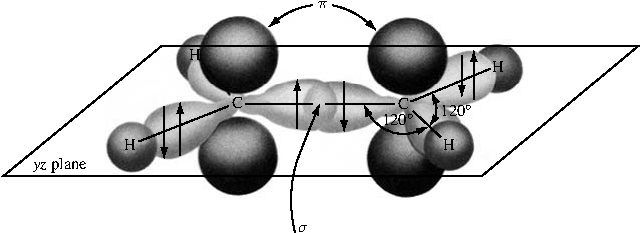
\includegraphics[width=0.8\textwidth]{Figures/ethylene.pdf}
\end{center}

The two \emph{$\pi$ electrons} are active (mobile), they can
jump from one C to the other: they are delocalized.
First, consider the $\pi$ electrons do not interact with each
other or with those $\sigma$ or with C; consider \emph{one} of the electrons

\begin{center}
$\pi$-bond: (C\textsubscript{2}H\textsubscript{2})\textsuperscript{++}\\[2ex]
\quad
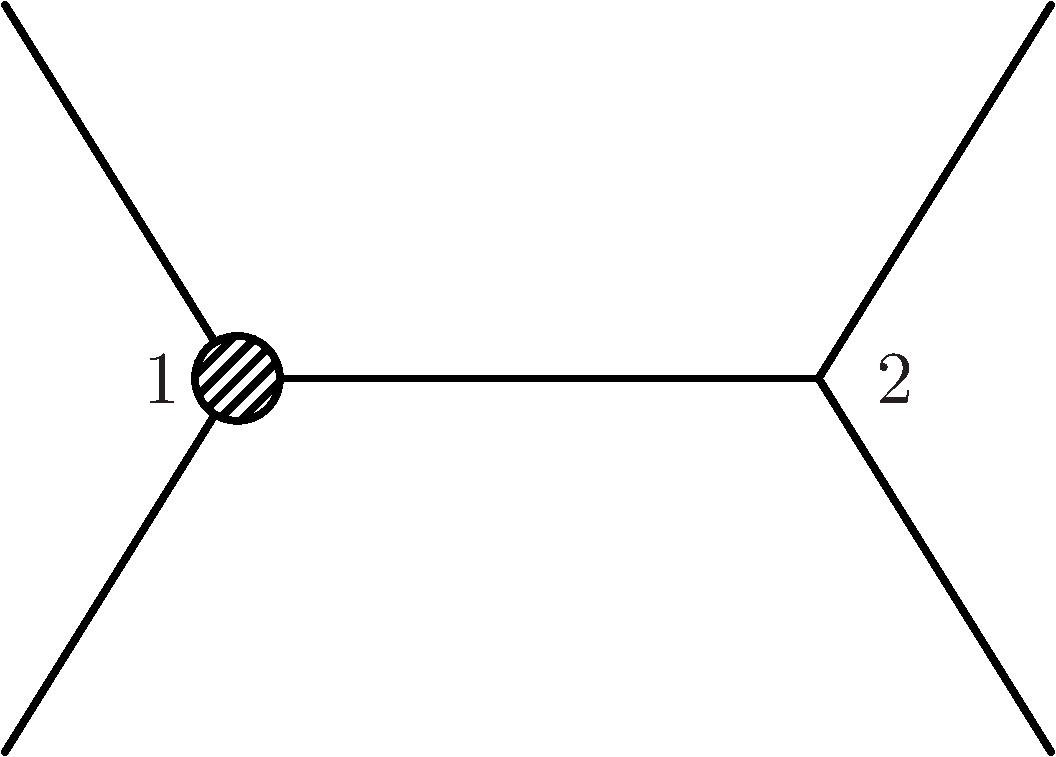
\includegraphics[width=0.4\textwidth]{Figures/electronAroundCAtom1.pdf}\hfill
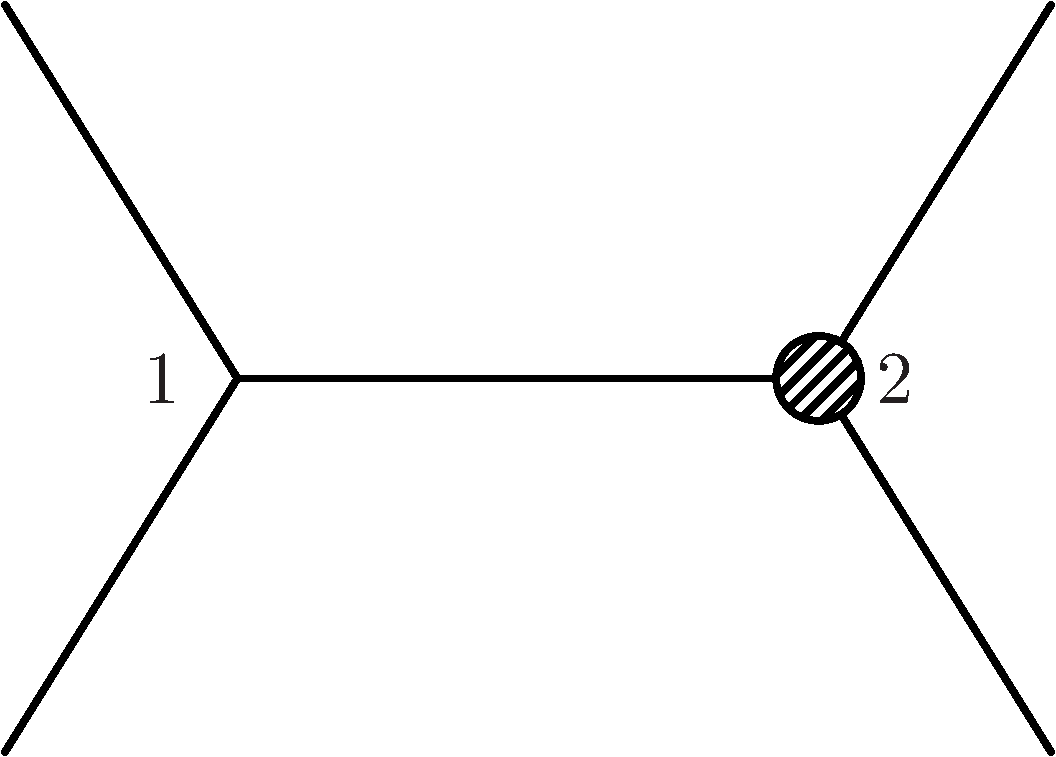
\includegraphics[width=0.4\textwidth]{Figures/electronAroundCAtom2.pdf}
\quad\\
Left: $\ket{\varphi_1}$ state, in which the electron is around C atom 1.
Right: $\ket{\varphi_2}$ state, in which the electron is around C atom 2.
\end{center}

%%% 2 OK

$H$ is two dimensional, $\{\ket{\varphi_1},\ket{\varphi_2}\}$ basis of the
noninteracting part $\hat{H}_0$:
\be
\hat{H}_{0}=\left(\begin{array}{cc}E_{0} & 0 \\ 0 & E_{0}\end{array}\right), 
\quad 
\hat{H}_{0}\left|\varphi_{1,2}\right\rangle=E_{0}\left|\varphi_{1,2}\right\rangle
\ee

Next, include interaction with C $\to$ electron can jump
\be
\hat{H}=\hat{H}_{0}+\hat{H}_{\text {int}}=
\left(\begin{array}{cc}E_{0} & -A \\ -A & E_{0}\end{array}\right),\quad A>0
\ee

$\ket{\varphi_1}$, $\ket{\varphi_2}$ are \emph{not} eigenstates of $\hat{H}$, but can
be used to expand the eigenstates $\to$ $\ket{\chi_{\pm}}$; can be seen in Chapter 2, Sec. 2.3.2 of Le~Bellac's book.
The symmetric $(1\leftrightarrow2)$ state:
\be
\begin{array}{l}
\left|\chi_{+}\right\rangle=\frac{1}{\sqrt{2}}\left[\left|\varphi_{1}\right\rangle
+
\left|\varphi_{2}\right\rangle\right]=\frac{1}{\sqrt{2}}
\left(\begin{array}{l}1 \\ 1\end{array}\right) \\ 
\hat{H}\left|\chi_{+}\right\rangle=E_{+}\left|\chi_{+}\right\rangle, E_{+}=E_{0}-A
\end{array}
\ee
and
the antisymmetric $(1\leftrightarrow2)$ state:
\be
\begin{array}{l}
\left|\chi_{-}\right\rangle=\frac{1}{\sqrt{2}}\left[\left|\varphi_{1}\right\rangle
-
\left|\varphi_{2}\right\rangle\right]=\frac{1}{\sqrt{2}}
\left(\begin{array}{l}\phantom{-}1 \\ -1\end{array}\right) \\ 
\hat{H}\left|\chi_{-}\right\rangle=E_{-}\left|\chi_{-}\right\rangle, E_{-}=E_{0}+A
\end{array}
\ee
so $\ket{\chi_+}$, the symmetric state, has the lowest energy.

\begin{center}
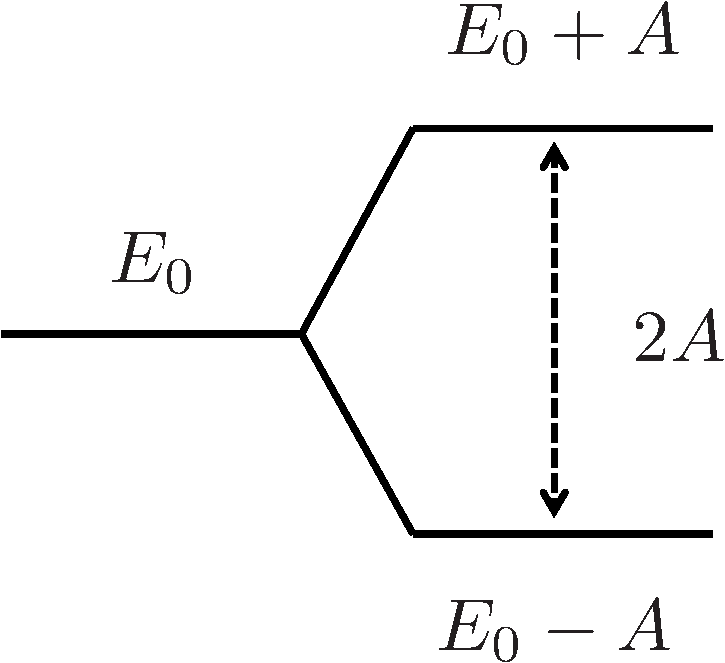
\includegraphics[width=0.3\textwidth]{Figures/twoStates.pdf}
\end{center}

Later on: $\varphi_{1,2} = \bra{x}\ket{\varphi_{1,2}}$, 
$\chi_{1,2} = \bra{x}\ket{\chi_{1,2}}$ will be the wavefunctions (see next page).
\clearpage

%%% 3 OK

\begin{center}
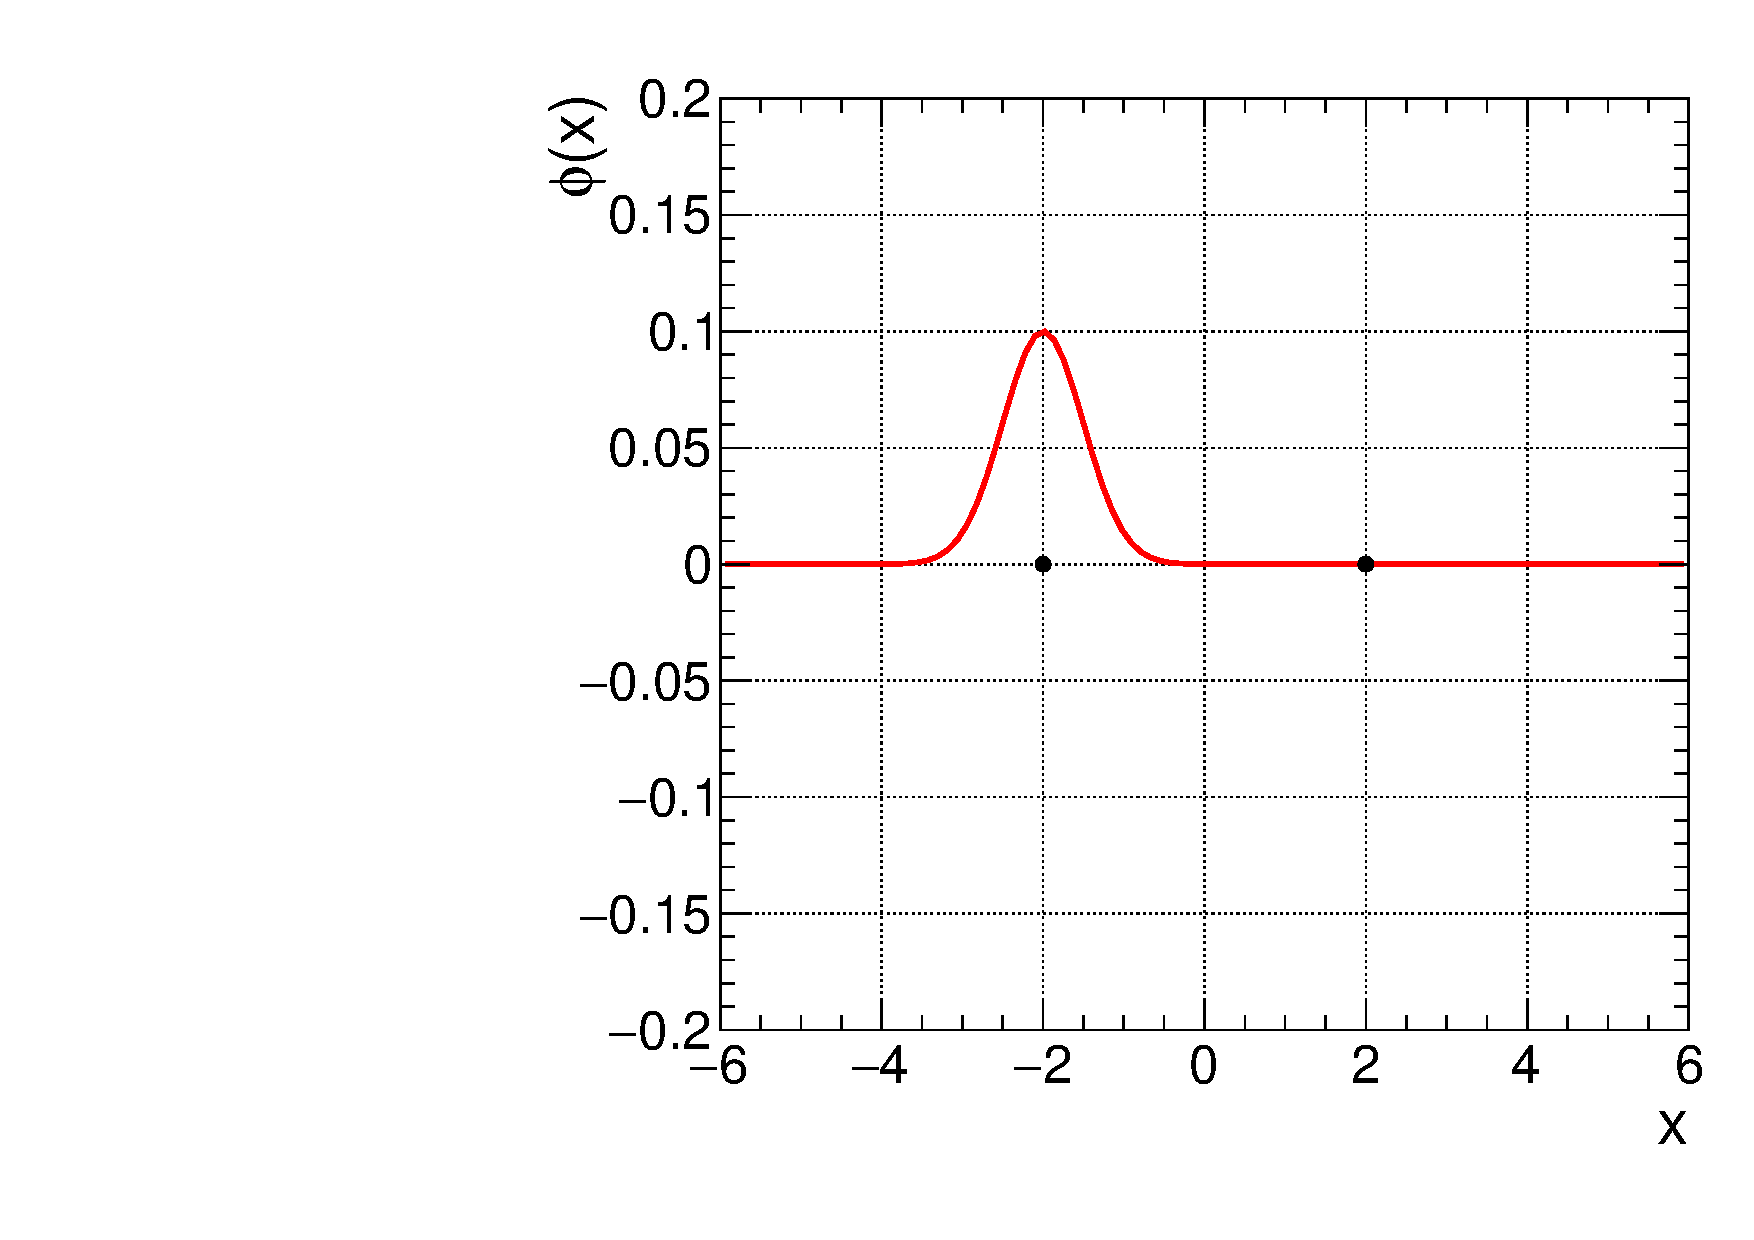
\includegraphics[width=0.44\textwidth]{Figures/phi1.pdf}
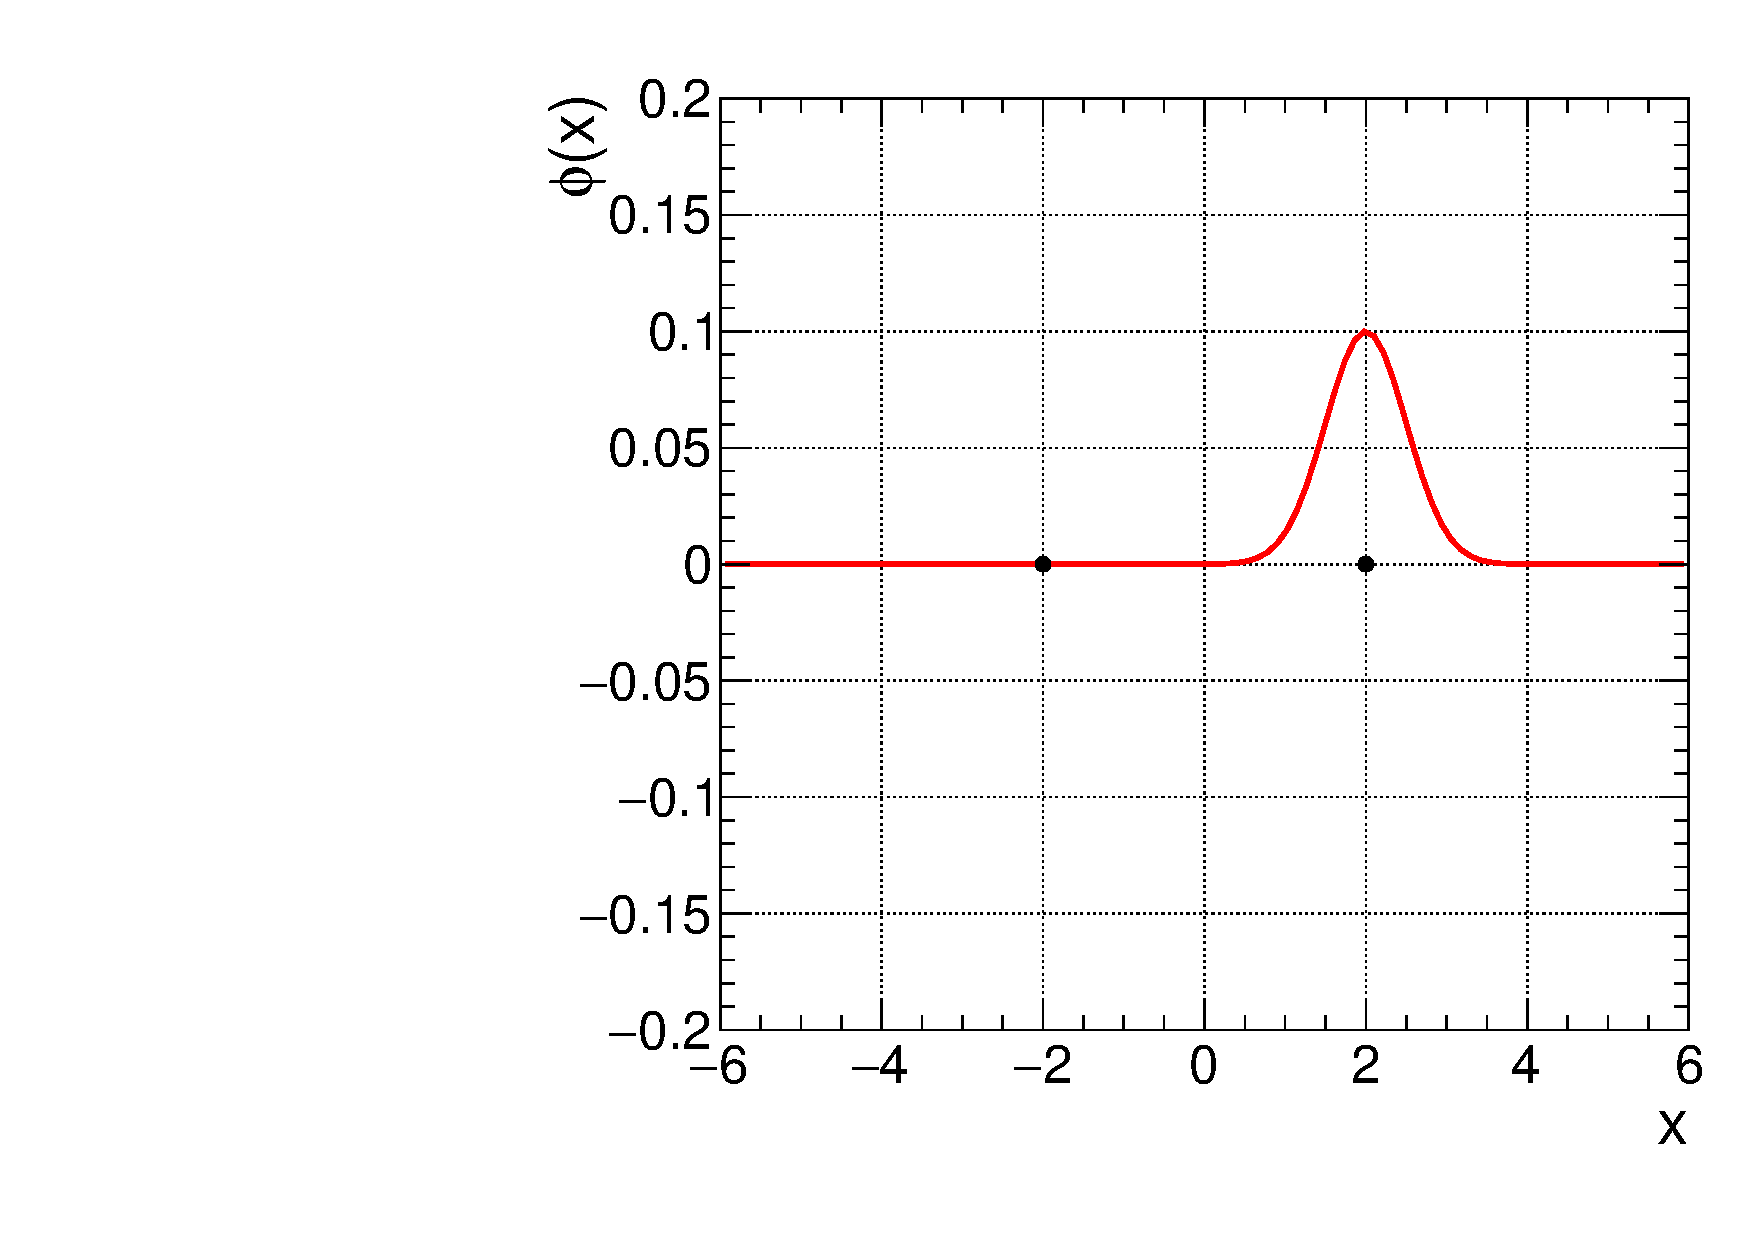
\includegraphics[width=0.45\textwidth]{Figures/phi2.pdf}\\
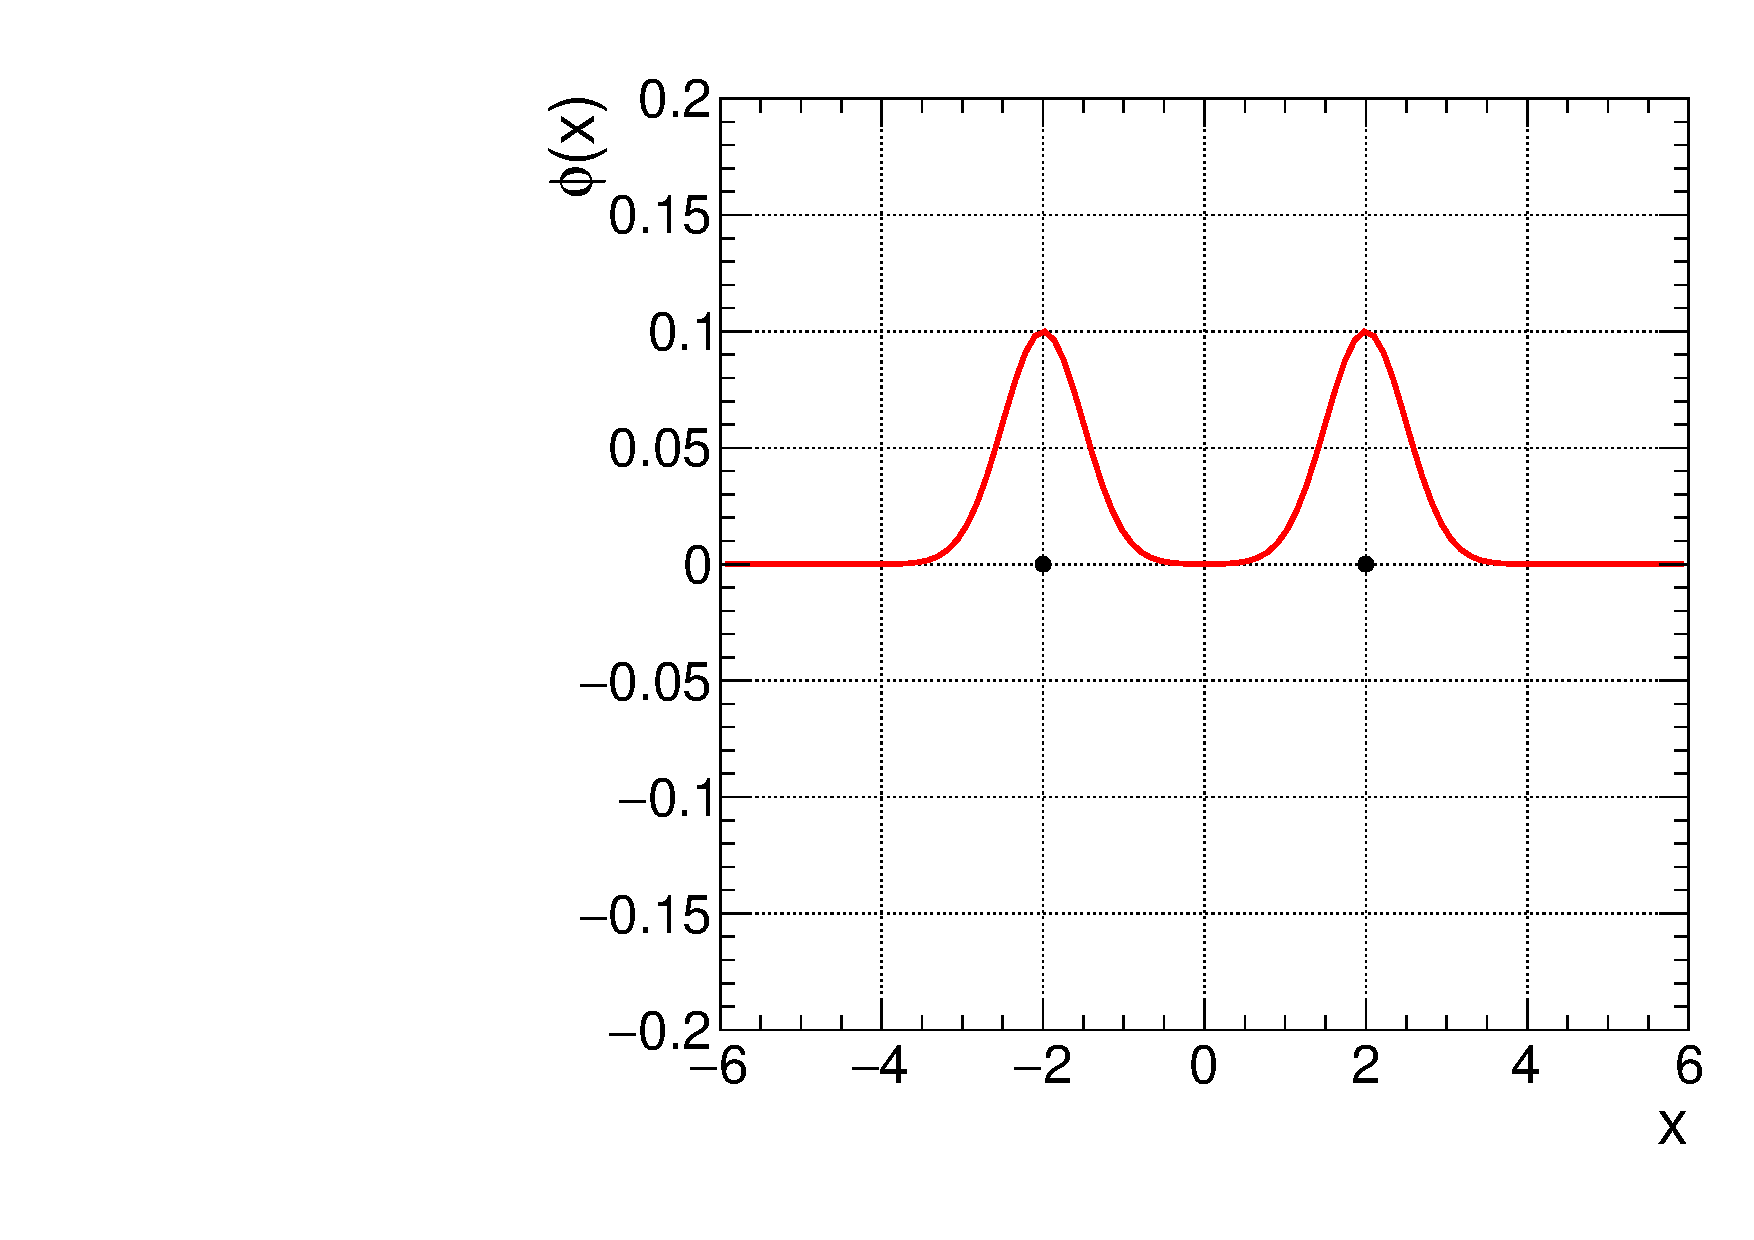
\includegraphics[width=0.45\textwidth]{Figures/chiPlus.pdf}
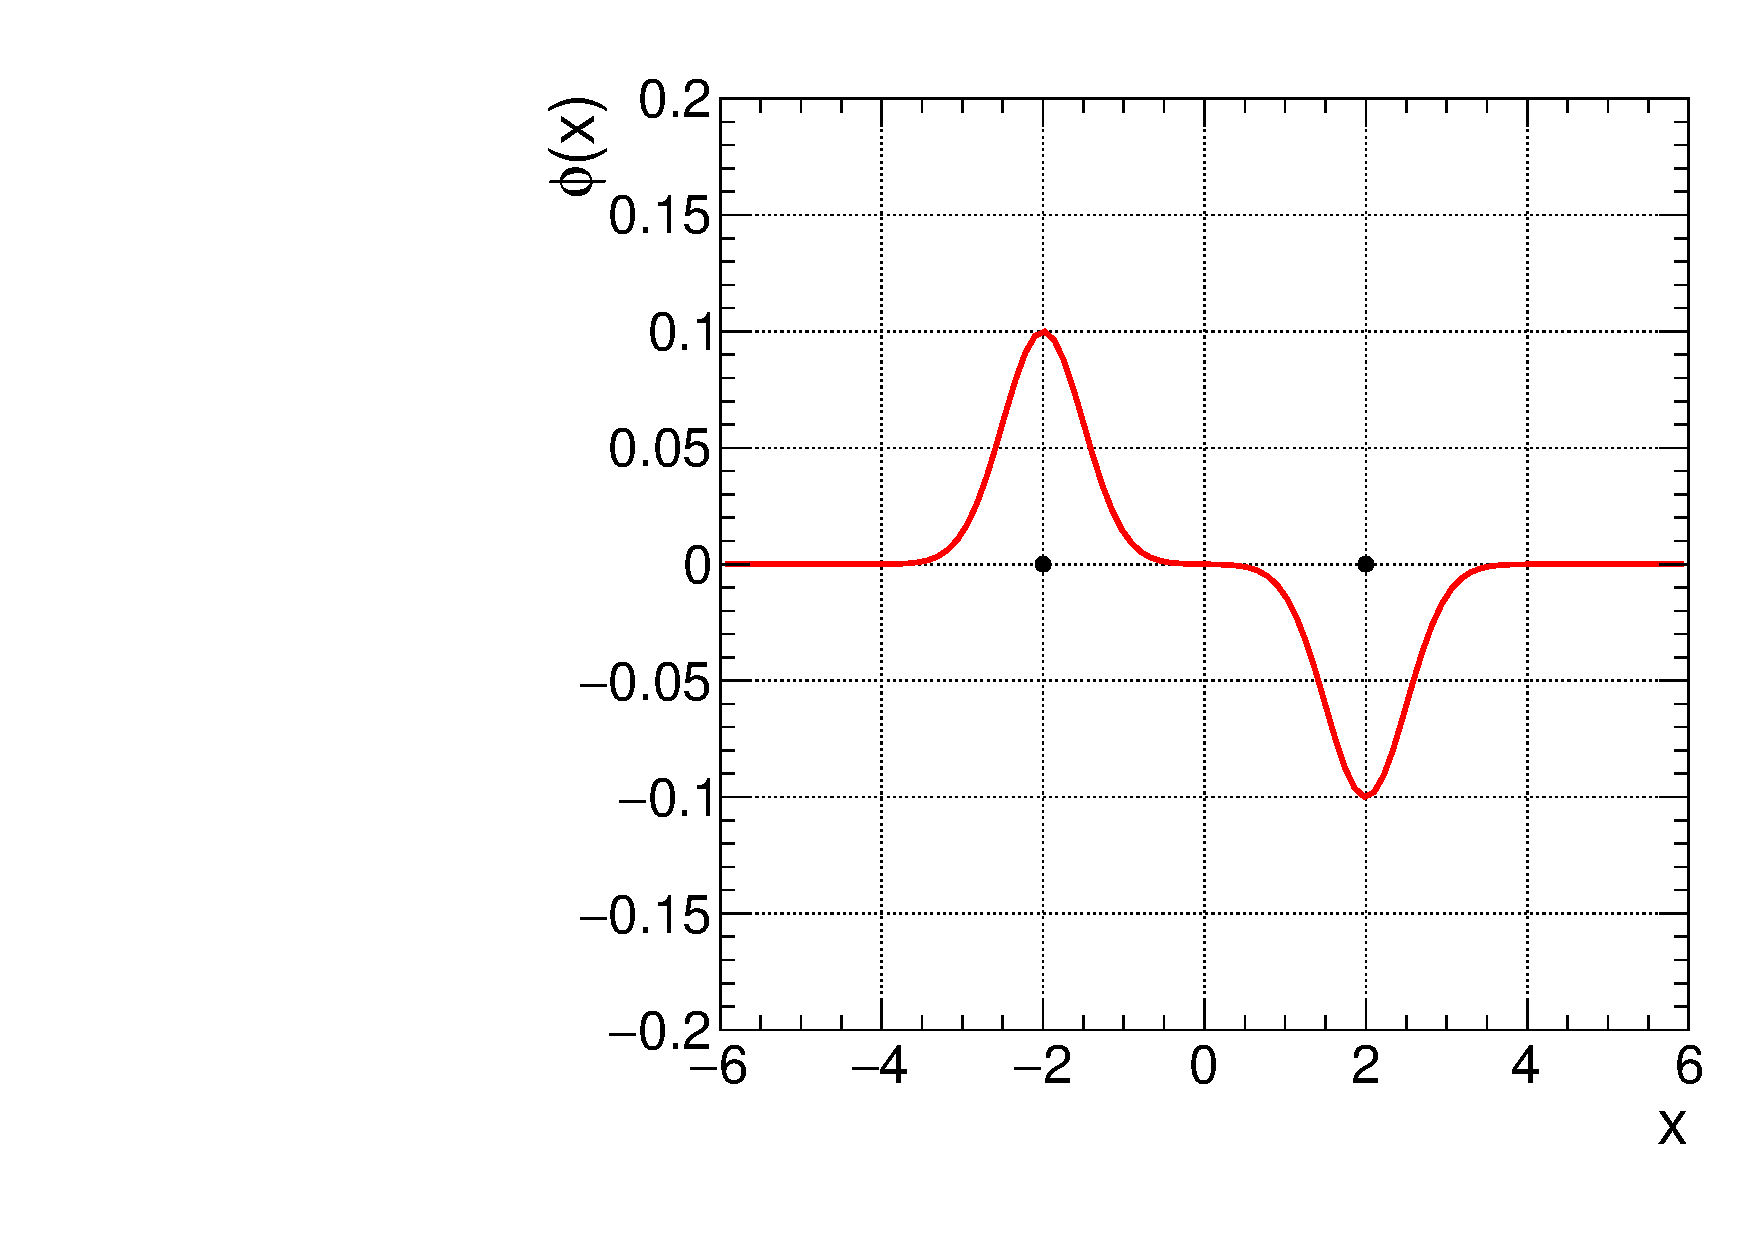
\includegraphics[width=0.45\textwidth]{Figures/chiMinus.pdf}
\end{center}
Top left: One-electron $\varphi_{1}$ function around carbon 1.
Top right: One-electron $\varphi_{2}$ function around carbon 2.
Bottom left: Two-electrons symmetric $\chi_{+}$ function.
Bottom right: Two-electrons antisymmetric $\chi_{-}$ function.


Now we include the second electron, but consider they
do not interact with each other 
$\to$ care must be taken with the Pauli principle.
Ground state: put the two in $\ket{\chi_{+}}$, with
total \emph{spin 0}, as the total wavefunction
must be antisymmetric:
\[
\frac{1}{\sqrt{2}}
\left(
\uparrow \downarrow-\downarrow \uparrow
\right)
\]
The energy of the $\pi$-bond is then $2(E_0-A)$; 
$-2A$ is the delocalization energy.
\emph{Note:} severe approximation, independent particle
approximation $\to$ no interactions between the
$\pi$ electrons or between $\pi$ and $\sigma$ electrons 
$\to$ even so, good starting point. 

%%% 4 OK

\subsection{Benzene molecule: $C_6H_6$}

\begin{center}
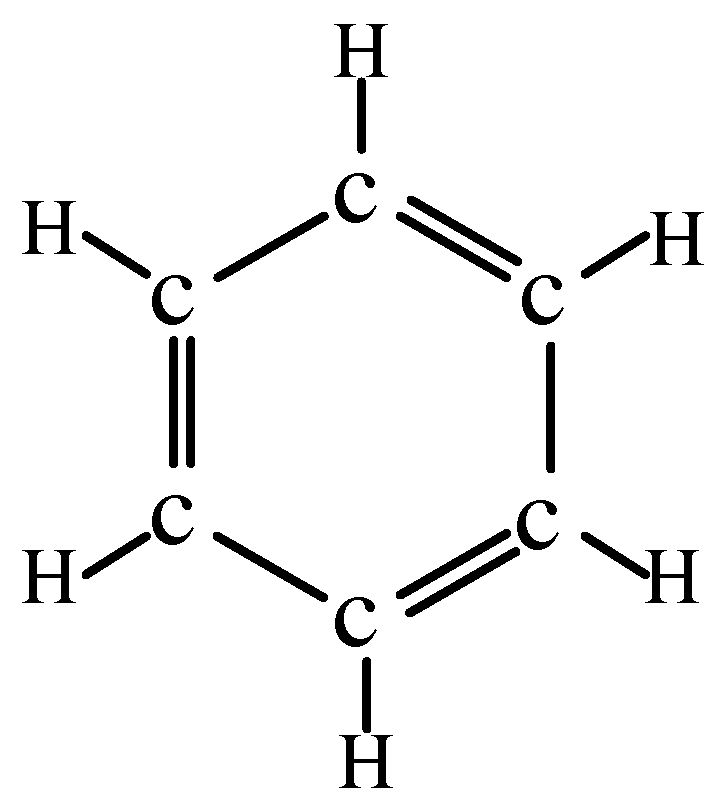
\includegraphics[width=0.3\textwidth]{Figures/benzene.pdf}
\end{center}
Removing the hydrogen electrons, we have the $(C_6H_6)^{6+}$ ion
with 3 $\pi$-bonds, represented by a double bar ($=\joinrel=\joinrel=$).
As in previous example: $6\times(E_0-A)$ ground state energy,
and $-6A$ delocalization energy: takes into account
delocalization \emph{between two $C$ atoms only}.
A better approximation is made when taking into
account delocalization over the entire chain.

Generalization: $6 \to N$ $C$ atoms.
$\ket{\varphi_n}$: (noninteracting) state near $n$-th atom,
$n=0,1,\ldots,N-1$.
Impose periodic boundary conditions: atoms $n$ and $n+N$
are identical. Let
$\{\ket{\varphi_0},\ldots,\ket{\varphi_{N-1}}\}$ be a basis in $H$, with dim. $N$. 
In this basis, the hamiltonian is the block-diagonal matrix
%%% 5 OK
\[
H=
\left(
\begin{array}{rrrrrr}
 E_{0} & -A & 0 & 0 & 0 & 0 \\ 
-A & E_{0} & -A & 0 & 0 & 0 \\ 
0 & -A & E_{0} & -A & 0 & 0 \\ 
0 & 0 & -A & E_{0} & -A & 0 \\ 
0 & 0 & 0 & -A & E_{0} & \ldots \\
\vdots & \vdots & \vdots& \vdots & \vdots & \ddots \\
\end{array}
\right)
\]

\be
\hat{H}\left|\varphi_{n}\right\rangle=E_{0}\left|\varphi_{n}\right\rangle-A\left(\left|\varphi_{n-1}\right\rangle+\left|\varphi_{n+1}\right\rangle\right)
\label{eq:g5}
\ee

Let $\hat{U}_{p},\,\hat{U}_{p}^{\dagger}=U_{p}^{-1}$: performs a permutation (hopping).
\be
\begin{array}{l}
\hat{U}_{p}\left|\varphi_{n}\right\rangle=\left|\varphi_{n-1}\right\rangle \\ 
\hat{U}_{p}^{\dagger}\left|\varphi_{n}\right\rangle=\hat{U}_{p}^{-1}\left|\varphi_{n}\right\rangle=\left|\varphi_{n+1}\right\rangle
\end{array}
\ee
so Eq.~\ref{eq:g5} can be written as
\[
\hat{H}\left|\varphi_{n}\right\rangle=E_{0} |\varphi_{n}\rangle-A\left(\hat{U}_{p}+\hat{U}_{p}^{\dagger}\right)\left|\varphi_{n}\right\rangle
\]
which implies
\be
\hat{H}=E_{0}-A\left(\hat{U}_{p}+\hat{U}_{p}^\dagger\right)
\ee
and therefore
\be
\left[\hat{H}, \hat{U}_{p}\right]=\left[\hat{H}, \hat{U}_{p}^{\dagger}\right]=0
\ee
$\hat{H}, \hat{U}_{p}$: basis of common eigenvectors.
Since $\hat{U}_{p}$ is simpler than $\hat{H}$, let us look for its
eigenvalues and eigenvectors. Since $\hat{U}_p$ is unitary
eigenvalues 
$\sim e^{i\delta}$, 
\[\underbrace{\hat{U}_{p}\,\ldots\,\hat{U}_{p}}%
_{N\textrm{ times}}
\left|\varphi_{n}\right\rangle=
\underbrace{\left|\varphi_{n-N}\right\rangle}%
_{|\varphi_{n}\rangle}
\]

%%% 6 OK
\be
\left(\hat{U}_{p}\right)^{N}\left|\varphi_{n}\right\rangle=\left|\varphi_{n}\right\rangle
\quad\therefore\quad
\left(\hat{U}_{p}\right)^{N}=I
\ee
so
\be
e^{i N \delta}=1 \quad N \delta=2 \pi s \quad s=0,1, \ldots, N-1
\ee
and
\be
\delta \rightarrow \delta_{s}=\frac{2\pi}{N} s, \quad s=0, \ldots, N-1
\ee
are $N$ distinct eigenvalues.
So $\hat{U}_{p}+\hat{U}_{p}^{\dagger}$ is Hermitian, orthonormal basis in $H$.

Let $\ket{\chi_s}$ be a common eigenvector of $\hat{H}$ and $\hat{U}_p$:
\be
\left|\chi_s\right\rangle=\sum_{n=0}^{N-1} C_{n}\left|\varphi_{n}\right\rangle
\quad,\quad
\sum_{n=0}^{N-1}\left|C_{n}\right|^{2}=1
\ee
So:
\begin{enumerate}
\item %
\be
\begin{aligned} 
\hat{U}_{p}\left|\chi_{s}\right\rangle 
&=\sum_{n=0}^{N-1} C_{n} \hat{U}_{p}\left|\varphi_{n}\right\rangle
=\sum_{n=0}^{N-1} C_{n}\left|\varphi_{n-1}\right\rangle \\ &=\sum_{m=-1}^{N-2} C_{m+1}\left|\varphi_{m}\right\rangle
=\sum_{n=0}^{N-1} C_{n+1}\left|\varphi_{n}\right\rangle \end{aligned}
\ee
\item%
\[
\hat{U}_{p}\left|\chi_{s}\right\rangle=e^{i \delta_{s}}\left|\chi_{s}\right\rangle=\sum_{n=0}^{N-1} e^{i \delta_{s}} C_{n}\left|\varphi_{n}\right\rangle
\]
\end{enumerate}
%
So, from those two 
\be
\begin{aligned}
C_{n+1} &= e^{i\delta_s} C_n\\
&=e^{i \delta_{s}}e^{\delta_{s}}C_{n-1}
=e^{i \delta_{s}} e^{i \delta_{s}} e^{i \delta_{s}} C_{n-2}\\
&=\underbrace{e^{i \delta_{s}} \ldots e^{i \delta_{s}}}%
_{n+1}  C_{0}=e^{i(n+1) \delta_{s}} C_{0}
\end{aligned}
\ee
%%% 7 OK
Therefore
\be
C_{n}=e^{i n \delta_{s}} C_{0}
\ee
and the eigenvector corresponding to
eigenvalue $e^{i\delta_s}$ is:
\[
\begin{aligned}
|\chi_{s}\rangle &=\sum_{n=0}^{N-1} C_{n} 
|\varphi_{n}\rangle=\sum_{n=0}^{N-1} C_{0} e^{i n \delta_{s}}\left|\varphi_{n}\right\rangle \\ &=C_{0} \sum_{n=0}^{N-1} e^{i n \delta_{s}}\left|\varphi_{n}\right\rangle 
\end{aligned}
\]
where
\be
\begin{gathered}
|C_{0}|^{2}+|C_{1}|^{2}+\ldots\left|C_{N-1}\right|^{2}=1=\left|C_{0}\right|^{2} \underbrace{(1+\cdots+1)}_{N}\\
\Rightarrow C_0 = \frac{1}{\sqrt{N}}
\end{gathered}
\ee
and finally
%%% 8 OK
\be
\boxed{
\left|\chi_{s}\right\rangle=\frac{1}{\sqrt{N}} \sum_{n=0}^{N-1} e^{i n \delta_{s}}\left|\varphi_{n}\right\rangle
}
\ee
with eigenvalue $\hat{H}\ket{\chi_s} = E_s\ket{\chi_s}$.
We calculate it explicitly:
\be
\begin{aligned} 
\hat{H}|\chi_s\rangle 
&=E_{0}|\chi_s\rangle-
A\left(\hat{U}_{p}+\hat{U}_{p}^{\dagger}\right)\left|\chi_s\right\rangle \\ 
&=\underbrace{\left[E_{0}-A\left(e^{i \delta_{s}}+e^{-i \delta_{s}}\right)\right]}%
_{E_{s}}
\left|\chi_s\right\rangle
\end{aligned}
\ee
hence
\[
\boxed{
E_{s}=E_{0}-2 A \cos \frac{2 \pi}{N} s
}
\quad,\quad s=0,1,\ldots,N-1
\]

\be
\text { Benzene: } N=6 \quad\
\left\{
\begin{aligned}
s=5: &\,E_{0}-2 A \cos 10 \pi / 6&=&\,E_{0}-A\\ 
s=4: &\,E_{0}-2 A \cos  8 \pi / 6&=&\,E_{0}+A\\ 
s=3: &\,E_{0}-2 A \cos    \pi / 6&=&\,E_{0}+2A\\ 
s=2: &\,E_{0}-2 A \cos  4 \pi / 6&=&\,E_{0}+A\\ 
s=1: &\,E_{0}-2 A \cos  2 \pi / 6&=&\,E_{0}-A\\ 
s=0: &\,E_{0}-2 A \cos  0 \pi / 6&=&\,E_{0}-2A
\end{aligned}
\right.
\ee
In general, $s$ and $N-s$ give same energy 
$\to$ $s\neq0$ double degenerate.

Ground state: approximation of independent electrons 
$\to$ Pauli principle;
\[
\text{6 electrons, $s\neq0$ double-degenerate}
\left\{
\begin{aligned}
&2\times(E_0-2A)\\
&4\times(E_0-A)
\end{aligned}
\right.
\]
so the energy of the ground state $E_\text{g.s.}$ is
\be
\begin{aligned} 
E_{\text {g.s.}} 
&=2\left(E_{0}-2 A\right)+4\left(E_{0}-A\right) \\ 
&=6 E_{0}-8 A=6\left(E_{0}-A\right)-2 A 
\end{aligned}
\ee
where the extra $-2A$ bit comes from
delocalization beyond
nearest-neighbouring atoms.

\emph{Note that:} since $s$ and $\tilde{s} = N-s$ give the
energy, with $\chi_{s} \neq \chi_{\tilde{s}}=\chi_{s}^{*}$, one can
%%% 9 OK
use their linear combinations to obtain 
eigenvectors with real components. Namely:
\be
\begin{aligned}
\left|\chi_s^{+}\right\rangle=\frac{1}{\sqrt{2}}\left(\left|\chi_s\right\rangle+\left|\chi_{\tilde{s}}\right\rangle\right)=\sqrt{\frac{2}{N}} \sum_{n=0}^{N-1} \cos \left(\frac{2 \pi n}{N} s\right)\left|\varphi_{n}\right\rangle\\
%
\left|\chi_s^{-}\right\rangle=\frac{1}{\sqrt{2}}\left(\left|\chi_s\right\rangle-\left|\chi_{\tilde{s}}\right\rangle\right)=\sqrt{\frac{2}{N}} \sum_{n=0}^{N-1} \sin \left(\frac{2 \pi n}{N} s\right)\left|\varphi_{n}\right\rangle
\end{aligned}
\ee
and we can finally write the six eigenvectors of benzene (left as exercise):
\be
\begin{aligned}
& s = 0,\,E = E_0 - 2A &
s = 1,\,\tilde{s}=5,\,E = E_0 - A\quad\quad\quad\quad\\
&\left|\chi_{0}\right\rangle=\frac{1}{\sqrt{6}}
\begin{pmatrix}1 \\ 1 \\ 1 \\ 1 \\ 1 \\ 1\end{pmatrix} & 
\left|\chi_{1}^+\right\rangle=\frac{1}{\sqrt{3}}
\begin{pmatrix}1 \\ 1/2 \\ -1/2 \\ -1 \\ -1/2 \\ 1/2\end{pmatrix}
\quad
\left|\chi_{1}^-\right\rangle=\frac{1}{\sqrt{3}}
\begin{pmatrix}0 \\ 1/2 \\ 1/2 \\ 0 \\ -1/2 \\ -1/2\end{pmatrix}
\end{aligned}
\ee
and for the others, see Le~Bellac's book.


\emph{Nuclear magnetic resonance} -- time dependence.
Next, time-dependent Hamiltonian, two-level
systems driven by an external \emph{classical} field
which is periodic with frequency $\omega$
$\to$ no stationary states, transitions between levels.

\end{document} 